\documentclass[11pt,a4paper]{article}
\usepackage[T1]{fontenc}
\usepackage[utf8]{inputenc}
\usepackage[margin=26mm,headheight=14pt]{geometry}
\usepackage{amsmath,amsthm,mathtools}
\usepackage{newtxtext,newtxmath}
\usepackage{microtype,booktabs,array,graphicx}
\usepackage{enumitem}
\usepackage[dvipsnames]{xcolor}
\usepackage{fancyhdr}
\usepackage{xurl}
\usepackage[colorlinks=true,linkcolor=MidnightBlue,citecolor=MidnightBlue,urlcolor=MidnightBlue,
  pdftitle={Complete Superconvergence Phases and Optimal Phase Filters for Rvachev Quadrature},
  pdfauthor={Research manuscript prepared with ChatGPT},
  pdfsubject={Quantitative phase classification, arithmetic rigidity, and sharp finite-filter bounds}]{hyperref}
\usepackage[capitalise,noabbrev]{cleveref}
\setlength{\parskip}{2pt}
\setlength{\parindent}{1.2em}
\setlist{itemsep=3pt,topsep=5pt}
\pagestyle{fancy}
\fancyhf{}
\fancyhead[L]{\small Rvachev quadrature: phases and filters}
\fancyhead[R]{\small Research manuscript}
\fancyfoot[C]{\thepage}
\renewcommand{\headrulewidth}{0.3pt}
\numberwithin{equation}{section}
\theoremstyle{plain}
\newtheorem{theorem}{Theorem}[section]
\newtheorem{lemma}[theorem]{Lemma}
\newtheorem{proposition}[theorem]{Proposition}
\newtheorem{corollary}[theorem]{Corollary}
\theoremstyle{definition}
\newtheorem{definition}[theorem]{Definition}
\newtheorem{example}[theorem]{Example}
\theoremstyle{remark}
\newtheorem{remark}[theorem]{Remark}
\newcommand{\R}{\mathbb R}
\newcommand{\C}{\mathbb C}
\newcommand{\Z}{\mathbb Z}
\newcommand{\N}{\mathbb N}
\newcommand{\T}{\mathbb T}
\newcommand{\dd}{\,\mathrm d}
\newcommand{\ii}{\mathrm i}
\newcommand{\sinc}{\operatorname{sinc}}
\newcommand{\supp}{\operatorname{supp}}
\newcommand{\ord}{\operatorname{ord}}
\newcommand{\dist}{\operatorname{dist}}
\newcommand{\vTwo}{\nu_2}
\newcommand{\Poly}{\mathcal P}
\newcommand{\lc}{\operatorname{lc}}
\newcommand{\repo}{\texttt{ProveIt}}
\newcommand{\code}[1]{\texttt{\small #1}}
\newcommand{\signedB}{B_M}
\newcommand{\baseharm}{\tau_p}
\newcommand{\absB}{A_M}

\begin{document}
\begin{titlepage}
\centering
\vspace*{12mm}
{\small\scshape Analysis / Fabius function / Rvachev up-function\par}
\vspace{13mm}
{\LARGE\bfseries Complete Superconvergence Phases\par}
\vspace{3mm}
{\LARGE\bfseries and Optimal Phase Filters\par}
\vspace{3mm}
{\LARGE\bfseries for Rvachev Quadrature\par}
\vspace{9mm}
{\large A quantitative completion of a ProveIt research frontier\par}
\vspace{10mm}
{Research manuscript prepared with ChatGPT\par}
{28 September 2026\par}
\vspace{12mm}
\begin{minipage}{0.92\textwidth}
\begin{abstract}
The ProveIt Fabius-function project establishes polynomial quadrature
exactness at parity-selected lattice phases, while explicitly leaving open
whether other first-superconvergent phases exist. We prove that they do not.
For every positive integer mesh parameter $M$, write $d=\nu_2(M)$.
Exactly two phases modulo one integrate all polynomials through degree
$d+1$: $0,\tfrac12$ when $d$ is even, and $\tfrac14,\tfrac34$ when $d$ is odd.
The proof is quantitative. An odd-multiplier inequality for the Fourier
product makes the entire first defect a relative perturbation of one
harmonic by at most $\pi^2/8-1<0.234$, uniformly in the odd part of $M$.
We also classify every finite complex phase measure giving polynomial
exactness uniformly under translation. At a reduced rational mesh $a/b$,
exactness through degree $r$ is equivalent to invariance under translation
by $1/(b2^{\max(0,r-\nu_2(a))})$. At an irrational mesh, even uniform
constant exactness forces Haar measure. The classification gives sharp
phase-count bounds, unique minimum-size filters up to translation, a finite
Fourier-moment recognition theorem, and corresponding results for
moment-deconvolved polynomial synthesis. Complete analytic proofs, exact
sample checks, and a further-research program are included.
\end{abstract}
\end{minipage}
\vfill
\begin{minipage}{0.92\textwidth}
\small
\textbf{Status.} The results below are proved in ordinary mathematics; no new
Lean or Rocq verification is claimed. Their novelty is assessed relative to
the specifically inspected repository statements and primary references,
not certified against the entire literature. This is an unrefereed research
manuscript, not a claim to have solved a major named conjecture.
\end{minipage}
\end{titlepage}

\begingroup
\small
\setlength{\parskip}{0pt}
\tableofcontents
\endgroup
\newpage

\section{The question and the precise contribution}
\label{sec:introduction}

A lattice quadrature can have greater polynomial exactness at a special
translation than at a generic translation. The central question here is
whether the familiar symmetry-selected translations of Rvachev quadrature
are the \emph{only} ones. A second question asks how efficiently several
translated copies can be combined to obtain exactness at \emph{every}
translation. These are different problems, and keeping their quantifiers
separate is essential.

Let $u$ be the normalized Rvachev up-function, supported on $[-1,1]$ and
satisfying $\int_\R u=1$. For a mesh parameter $M>0$ and a phase
$\theta\in\T=\R/\Z$, put
\begin{equation}\label{eq:quadrature}
 Q_{M,\theta}(P)=\frac1M\sum_{k\in\Z}
 P\!\left(\frac{k+\theta}{M}\right)
 u\!\left(\frac{k+\theta}{M}\right),
 \qquad I(P)=\int_\R P(x)u(x)\dd x.
\end{equation}
The actual lattice spacing is $1/M$. The sum is finite because $u$ is
compactly supported. We write $\Poly_r$ for the complex polynomials of
degree at most $r$, including the zero polynomial.

The source module \code{RvachevSuperconvergentSynthesis.lean}
proves that, for $M\in\N_{>0}$, every phase is exact on
$\Poly_{\nu_2(M)}$, and the indicated parity-selected phases are exact on
$\Poly_{\nu_2(M)+1}$. Its introductory documentation explicitly disclaims
completeness of that phase list. The module
\code{CombDefectSeries.lean} supplies the absolutely convergent Fourier
series for the defect and its odd-frequency support at the first failing
degree \cite{repo-phase,repo-defect}.

The repository reference used here is the commit
\begin{center}
\small\texttt{de4ac5ab1438bcbeed58481c4449b593074a1a1f}.
\end{center}
We inspected the relevant module statements, proof portions, and frontier
overview, not every research artifact in the repository. The classical
function, its Fourier-product description, and its dyadic arithmetic are
not new; primary references include Arias de Reyna
\cite{arias1982,arias2017}. The use of Fourier zeros to control polynomial
reproduction belongs to the Strang--Fix tradition; see, for example,
Zakharov \cite{zakharov2013}. Our contribution is the specific quantitative
phase-completeness argument and the full phase-measure classification
worked out for this kernel.

\subsection{Results at a glance}

\Cref{thm:complete-phases} proves the missing necessity statement, for
\emph{all} positive integer $M$, not just powers of two. It also gives a
uniform relative error bound, the sign of the first defect, and simplicity
of its two zeros. The key ingredient is the estimate
\[
 \left|H\!\left(\frac{ak}{2}\right)\right|
 \le \frac1{k^2}\left|H\!\left(\frac a2\right)\right|
 \qquad(a,k\text{ positive odd}),
\]
where $H=\widehat u$. The estimate retains the odd part $a$ of the mesh;
it does not replace it by a mesh-dependent unspecified constant.

\Cref{thm:measure-classification} identifies every mass-one finite complex
measure on the phase circle that is uniformly exact through a prescribed
degree. The answer is an exact cyclic-invariance condition at rational
meshes and a Haar-measure rigidity statement at irrational meshes.
\Cref{thm:fixed-count,thm:budget} then solve the finite phase-budget problem,
including its equality cases. Negative or complex weights do not improve
the bound. \Cref{thm:finite-recognition} turns cyclic invariance of a real
signed atomic filter into a finite set of Fourier-moment tests.

Finally, \Cref{thm:synthesis} transfers the results to polynomial synthesis
after moment deconvolution. Exact rational computations and numerical
product checks provide independent diagnostics, not substitutes for the
proofs.

\subsection{What the statements do not assert}

The phase theorem classifies exactness through the \emph{first additional}
degree $\nu_2(M)+1$. It does not prove that every selected phase necessarily
fails at the next degree $\nu_2(M)+2$. That separate fixed-phase maximality
problem remains in the research program. Conversely, our finite-filter
maximality theorem is complete, but concerns exactness \emph{uniformly in
the translating phase}. It is not a lower bound for unrestricted Gaussian
quadrature or for arbitrary node placement at a single fixed phase.

\section{Normalization, Fourier zeros, and the defect series}
\label{sec:preliminaries}

\subsection{A construction fixing all factors of two}

Take independent random variables $V_j$, each uniform on $[-1,1]$, and set
\begin{equation}\label{eq:probability}
 Y=\sum_{j=1}^{\infty}2^{-j}V_j.
\end{equation}
The sum converges absolutely and lies in $[-1,1]$. With the convention
\[
 \widehat f(t)=\int_\R f(x)e^{-2\pi\ii tx}\dd x,
 \qquad \sinc z=\begin{cases}\sin z/z,&z\ne0,\\1,&z=0,\end{cases}
\]
its characteristic function is
\begin{equation}\label{eq:Hproduct}
 H(t)=\prod_{j=0}^{\infty}\sinc\!\left(\frac{\pi t}{2^j}\right).
\end{equation}
This choice of $Y$ is important: starting the product at $j=1$ instead would
change the support and every mesh convention.

For every compact subset of $\C$, the tail factors differ from $1$ by
$O(4^{-j})$, uniformly on that subset. Hence the product defines an entire
function. On the real axis each factor has absolute value at most one.
For any $N$, bounding the first $N$ factors by their reciprocal arguments
shows that $H(t)=O_N(|t|^{-N})$ as $|t|\to\infty$. Fourier inversion thus
gives a $C^\infty$ density $u$ of the law of $Y$. It is even, nonnegative,
has integral one, and vanishes outside $[-1,1]$. Its compact support and
smoothness imply that $H$ and all its derivatives are Schwartz functions
on $\R$.

The first summand in \eqref{eq:probability} is uniform on
$[-\tfrac12,\tfrac12]$, with density one. The remaining sum has support in
the same interval and has no endpoint atoms. Convolution therefore gives
$u(0)=1$. This is the conventional normalization used in the cited
Rvachev-function literature and in the repository.

\begin{lemma}[Complete real zero set and multiplicity]\label[lemma]{lem:zeros}
The real zeros of $H$ are exactly the nonzero integers. For
$n\in\Z\setminus\{0\}$,
\begin{equation}\label{eq:zero-order}
 \ord_n H=\nu_2(|n|)+1.
\end{equation}
In particular, $H(a/2)\ne0$ for every odd integer $a$.
\end{lemma}
\begin{proof}
A factor in \eqref{eq:Hproduct} vanishes precisely when
$t$ is a nonzero multiple of $2^j$. If $t$ is a nonzero integer of
valuation $d$, exactly the factors $j=0,\ldots,d$ vanish, each simply.
All other factors are nonzero. Their product is also nonzero: after
finitely many factors, the sum of the absolute deviations from one
converges and the factors stay in a neighborhood of one. The same
nonvanishing argument applies when no factor vanishes. Thus no additional
zeros arise from the infinite tail, and the multiplicity is $d+1$.
\end{proof}

The zero structure itself is classical; it is also visible in the
canonical product in \cite[eq.~(9)]{arias1982}. We have given the short
factor argument to make clear which exact property is used below.

\subsection{Poisson summation in physical coordinates}

Define the monomial defect
\begin{equation}\label{eq:defect}
 E_{r,M}(\theta)=Q_{M,\theta}(x^r)-I(x^r),\qquad r\ge0.
\end{equation}
For a general polynomial, write $E_{P,M}=Q_{M,\theta}(P)-I(P)$ when the
phase is understood.

\begin{proposition}[Defect Fourier series]\label[proposition]{prop:poisson}
For every $M>0$ and integer $r\ge0$,
\begin{equation}\label{eq:poisson}
 E_{r,M}(\theta)=\left(\frac{\ii}{2\pi}\right)^r
 \sum_{k\in\Z\setminus\{0\}}H^{(r)}(Mk)e^{2\pi\ii k\theta}.
\end{equation}
The series and each of its phase derivatives converge absolutely and
uniformly.
\end{proposition}
\begin{proof}
The function $f_r(x)=x^r u(x)$ is smooth and compactly supported.
Its periodization is
\[
 g_r(\theta)=M^{-1}\sum_{j\in\Z} f_r((j+\theta)/M).
\]
This has $k$th Fourier coefficient $\widehat f_r(Mk)$: substitute
$x=(j+\theta)/M$ in the coefficient integral and join the resulting
intervals. Its Fourier coefficients decrease faster than any power.
Moreover,
\[
 H^{(r)}(t)=\int_\R(-2\pi\ii x)^r u(x)e^{-2\pi\ii tx}\dd x,
 \qquad \widehat f_r(t)=\left(\frac\ii{2\pi}\right)^r H^{(r)}(t).
\]
Removing the zero coefficient, which equals $I(x^r)$, proves
\eqref{eq:poisson}. Rapid decay also proves all the stated convergence
claims.
\end{proof}

\begin{corollary}[Uniform base order at an integer mesh]\label[corollary]{cor:base-order}
If $M\in\N_{>0}$ and $d=\nu_2(M)$, then $Q_{M,\theta}=I$ on
$\Poly_d$ at every phase. This uniform order is exactly $d$.
\end{corollary}
\begin{proof}
Every nonzero integer $Mk$ has zero multiplicity at least $d+1$ in $H$.
Thus all the terms in \eqref{eq:poisson} vanish for $r\le d$.
For $r=d+1$, the coefficient at $k=1$ is nonzero by
\cref{lem:zeros}, so the defect cannot vanish identically.
\end{proof}

The repository's unnormalized lattice-coordinate defect uses
$(k+\theta)^r u((k+\theta)/M)$ and the corresponding integral. It is
$M^{r+1}E_{r,M}(\theta)$. This observation reconciles
\eqref{eq:poisson} with the source-module statement and prevents an
otherwise easy normalization error.

\section{An odd-multiplier inequality and the first alias}
\label{sec:odd-multiplier}

\begin{lemma}[Integer-multiple sine bound]\label[lemma]{lem:sine}
For real $z$ and positive integer $k$,
\begin{equation}\label{eq:sine-bound}
 |\sin(kz)|\le k|\sin z|.
\end{equation}
For odd $k$, also $|\cos(kz)|\le k|\cos z|$.
\end{lemma}
\begin{proof}
The identity
\[
 e^{\ii kz}-e^{-\ii kz}
 =(e^{\ii z}-e^{-\ii z})
 \sum_{j=0}^{k-1}e^{\ii(k-1-2j)z}
\]
and the triangle inequality prove the sine estimate. For odd $k$,
replace $z$ by $z+\pi/2$ and take absolute values to obtain the cosine
estimate. The argument includes the points where the right side is zero.
\end{proof}

\begin{lemma}[Odd-multiplier domination]\label[lemma]{lem:odd-domination}
If $a,k$ are positive odd integers, then
\begin{equation}\label{eq:odd-domination}
 \frac{|H(ak/2)|}{|H(a/2)|}\le \frac1{k^2}.
\end{equation}
\end{lemma}
\begin{proof}
For each factor of \eqref{eq:Hproduct}, put
$z_j=\pi a/2^{j+1}$. None of $\sin z_j$ is zero. By
\cref{lem:sine},
\[
 \frac{|\sinc(kz_j)|}{|\sinc(z_j)|}
 =\frac{|\sin(kz_j)|}{k|\sin z_j|}\le1.
\]
The first two factors are stronger. Oddness gives
\[
 |\sin(\pi ak/2)|=|\sin(\pi a/2)|=1,
 \qquad
 |\sin(\pi ak/4)|=|\sin(\pi a/4)|=\frac1{\sqrt2}.
\]
Their ratios are therefore exactly $1/k$ each. For every finite product
containing those two factors, the full ratio is at most $k^{-2}$.
Pass to the limit, using $H(a/2)\ne0$ from \cref{lem:zeros}.
\end{proof}

\begin{remark}
A generic rapid-decay estimate bounds $H(ak/2)$ by an unspecified constant
that may be much larger than $|H(a/2)|$. Such an estimate cannot rule out
extra zeros when the first coefficient is small. The content of
\eqref{eq:odd-domination} is its comparison with the \emph{actual first
coefficient}, uniformly over every odd $a$.
\end{remark}

\begin{lemma}[Exact first nonzero alias]\label[lemma]{lem:first-alias}
Let $M=2^d a$ with $a$ positive odd, and put $p=d+1$. For odd
$k\in\Z\setminus\{0\}$,
\begin{equation}\label{eq:first-alias}
 H^{(p)}(Mk)=-\frac{p!}{(Mk)^p}H(ak/2).
\end{equation}
For nonzero even $k$, $H^{(p)}(Mk)=0$.
\end{lemma}
\begin{proof}
Write $n=Mk$. For odd $k$, separate the first $p$ factors:
\[
 H(t)=\left(\prod_{j=0}^{d}\sinc(\pi t/2^j)\right)H(t/2^{d+1}).
\]
At $t=n$, each of the displayed factors has a simple zero, with derivative
$(-1)^{n/2^j}/n$. In the $p$th derivative, only the term differentiating
every one of these factors once survives. Its combinatorial coefficient
is $p!$. Its sign is
\[
 (-1)^{\sum_{j=0}^d n/2^j}
 =(-1)^{ak(2^{d+1}-1)}=-1.
\]
The remaining factor is $H(ak/2)$, giving
\eqref{eq:first-alias}. The argument is valid for negative odd $k$ too.
For even $k$, \cref{lem:zeros} gives multiplicity at least $p+1$.
\end{proof}

Define the nonzero real number and the reference harmonic
\begin{equation}\label{eq:B-tau}
 B_M=-\frac{2p!}{(2\pi M)^p}H(a/2),\qquad
 A_M=|B_M|,\qquad
 \tau_p(\theta)=\cos(2\pi\theta+p\pi/2).
\end{equation}
Pairing $k$ and $-k$ in \eqref{eq:poisson} now yields the exact real series
\begin{equation}\label{eq:normalized-series}
 \frac{E_{p,M}(\theta)}{B_M}
 =\sum_{\substack{k\ge1\\k\text{ odd}}}
 \frac{H(ak/2)}{H(a/2)\,k^p}
 \cos(2\pi k\theta+p\pi/2).
\end{equation}
The sign in $B_M$ and the phase shift $p\pi/2$ should both be retained;
replacing this display by an unsigned amplitude would lose the defect's
orientation.

\section{The complete phase theorem and its stability estimates}
\label{sec:phase-theorem}

For $p\ge1$, put
\begin{equation}\label{eq:delta}
 \delta_p=\sum_{\substack{k\ge3\\k\text{ odd}}}k^{-(p+1)}
 =(1-2^{-(p+1)})\zeta(p+1)-1.
\end{equation}
Then $0<\delta_p\le\delta_1=\pi^2/8-1<1$. No evaluation of $\zeta$
is needed for the strict inequality: termwise comparison with
$1/(k(k-1))$ gives
\begin{equation}\label{eq:rational-delta}
 \delta_p\le\sum_{\substack{k\ge3\\k\text{ odd}}}\frac1{k^2}
 <\sum_{k=3}^\infty\frac1{k(k-1)}=\frac12.
\end{equation}
This weaker rational bound is sufficient for the classification.

\begin{theorem}[Complete first-superconvergent phases]\label{thm:complete-phases}
Let $M\in\N_{>0}$, $d=\nu_2(M)$, $p=d+1$, and $a=M/2^d$.
For every $\theta\in\T$,
\begin{equation}\label{eq:relative-main}
 \left|\frac{E_{p,M}(\theta)}{B_M}-\tau_p(\theta)\right|
 \le\delta_p|\tau_p(\theta)|.
\end{equation}
Consequently $Q_{M,\theta}=I$ on $\Poly_p$ if and only if
\begin{equation}\label{eq:phase-classification}
 \theta\in Z_p:=
 \begin{cases}
 \{0,\tfrac12\}\pmod1,&p\text{ odd},\\[2pt]
 \{\tfrac14,\tfrac34\}\pmod1,&p\text{ even}.
 \end{cases}
\end{equation}
There are exactly two such phases modulo one. Away from them,
$E_{p,M}/B_M$ has the same sign as $\tau_p$.
\end{theorem}
\begin{proof}
The $k=1$ term in \eqref{eq:normalized-series} is $\tau_p$.
For odd $k$, \cref{lem:sine} implies
\[
 |\cos(2\pi k\theta+p\pi/2)|\le
 k|\cos(2\pi\theta+p\pi/2)|.
\]
Indeed, for even $p$ this is the cosine inequality, and for odd $p$ it is
the sine inequality, with harmless signs. By
\cref{lem:odd-domination}, the remaining terms have total absolute value
at most
\[
 \sum_{\substack{k\ge3\\k\text{ odd}}}
 \frac{1}{k^{p+2}}\,k|\tau_p(\theta)|
 =\delta_p|\tau_p(\theta)|.
\]
This proves \eqref{eq:relative-main}. If $\tau_p(\theta)=0$, the bound
forces the defect to vanish. If $\tau_p(\theta)\ne0$, the ratio of
$E_{p,M}(\theta)/B_M$ to $\tau_p(\theta)$ lies in
$[1-\delta_p,1+\delta_p]\subset(0,\infty)$, so the defect is nonzero
and has the asserted sign. The zeros of $\tau_p$ are exactly
\eqref{eq:phase-classification}. Finally, all lower monomial defects
vanish by \cref{cor:base-order}; exactness on $\Poly_p$ is therefore
equivalent to vanishing of this one defect.
\end{proof}

\begin{corollary}[Simplicity, global phase conditioning, and polynomial errors]
\label[corollary]{cor:stability}
Under the hypotheses of \cref{thm:complete-phases},
\begin{equation}\label{eq:amplitude-bounds}
 (1-\delta_p)A_M|\tau_p(\theta)|
 \le |E_{p,M}(\theta)|
 \le (1+\delta_p)A_M|\tau_p(\theta)|.
\end{equation}
Every $\theta_0\in Z_p$ is a simple zero, and
\begin{equation}\label{eq:derivative-root}
 2\pi A_M(1-\delta_p)\le |E'_{p,M}(\theta_0)|
 \le2\pi A_M(1+\delta_p).
\end{equation}
For $\rho=\dist_{\T}(\theta,Z_p)\in[0,\tfrac14]$,
\begin{equation}\label{eq:distance-bound}
 4(1-\delta_p)A_M\rho\le |E_{p,M}(\theta)|
 \le2\pi(1+\delta_p)A_M\rho.
\end{equation}
If $P(x)=c_px^p+\cdots+c_0$, then
$Q_{M,\theta}(P)-I(P)=c_p E_{p,M}(\theta)$.
\end{corollary}
\begin{proof}
The first assertion follows immediately from
\eqref{eq:relative-main}. Termwise differentiation is justified either by
\cref{prop:poisson} or by
\[
 \sum_{\substack{k\ge3\\k\text{ odd}}}
 k\left|\frac{H(ak/2)}{H(a/2)k^p}\right|\le\delta_p.
\]
It gives the global estimate
\begin{equation}\label{eq:C1}
 \left|\left(E_{p,M}/B_M\right)'(\theta)-\tau'_p(\theta)\right|
 \le2\pi\delta_p.
\end{equation}
At a zero of $\tau_p$, the reference derivative has absolute value
$2\pi$, proving \eqref{eq:derivative-root} and simplicity.
Next, $|\tau_p(\theta)|=\sin(2\pi\rho)$. Concavity of sine on
$[0,\pi/2]$ and the bound $\sin t\le t$ give
$4\rho\le\sin(2\pi\rho)\le2\pi\rho$.
Combine this with \eqref{eq:amplitude-bounds}. The polynomial statement
uses the vanishing of every lower monomial defect.
\end{proof}

\subsection{Binary orientation and a uniform first-harmonic limit}

The sign of the amplitude can be computed without evaluating an infinite
product. Let $s_2(a)$ be the number of ones in the binary expansion of $a$.
For positive odd $a$,
\begin{equation}\label{eq:binary-sign}
 \operatorname{sgn} H(a/2)=(-1)^{s_2(a)-1},\qquad
 \operatorname{sgn} B_M=(-1)^{s_2(a)}.
\end{equation}
To check this, the sign of the $j$th sine factor is
$(-1)^{\lfloor a/2^{j+1}\rfloor}$, and
\[
 \sum_{j\ge0}\left\lfloor\frac a{2^{j+1}}\right\rfloor=a-s_2(a).
\]
The latter identity follows by expanding $a$ in binary and summing the
contribution $2^m-1$ of each nonzero digit in position $m$. Since $a$ is
odd, the claimed parity follows. This digital sign law is part of the
classical Fourier description; here it gives the orientation of the new
zero classification.

As $p\to\infty$, $\delta_p\to0$ by dominated convergence. Equations
\eqref{eq:relative-main} and \eqref{eq:C1} imply a $C^1$ first-harmonic
limit uniform over \emph{all} odd parts $a$ of the mesh. This is a relative
statement after normalization by $B_M$. It does not say that the absolute
amplitudes $A_M$ are bounded below uniformly in $M$ or $a$.

\begin{table}[htbp]
\centering
\caption{Uniform relative-tail bounds. The bound is independent of the odd
part of the mesh.}
\label{tab:delta}
\begin{tabular}{@{}crr@{}}
\toprule
$p=\nu_2(M)+1$ & $\delta_p$ & Guaranteed factor $1-\delta_p$\\
\midrule
1 & 0.233700550136 & 0.766299449864\\
2 & 0.051799790265 & 0.948200209735\\
3 & 0.014678031604 & 0.985321968396\\
4 & 0.004523762795 & 0.995476237205\\
5 & 0.001447076641 & 0.998552923359\\
\bottomrule
\end{tabular}
\end{table}

\section{All translation-uniform phase filters}
\label{sec:filters}

\subsection{Definition and a Fourier criterion}

Let $\mu$ be a finite complex Borel measure on $\T$ with
$\mu(\T)=1$. Its positive-sign Fourier coefficients are
\begin{equation}\label{eq:measure-fourier}
 c_\mu(k)=\int_{\T}e^{2\pi\ii k\phi}\dd\mu(\phi).
\end{equation}
Define the filtered quadrature
\begin{equation}\label{eq:filtered}
 Q^\mu_{M,\theta}(P)
 =\int_{\T}Q_{M,\theta+\phi}(P)\dd\mu(\phi).
\end{equation}
The atomic case $\mu=\sum_{j=1}^N w_j\delta_{\phi_j}$ is a weighted
average of $N$ translated quadratures, with $\sum_jw_j=1$. The weights
need not be positive or real.

\begin{definition}[Uniform exactness]\label[definition]{def:uniform}
The filter $\mu$ is uniformly exact through degree $r$ at mesh $M$ if
\[
 Q^\mu_{M,\theta}(P)=I(P)
 \quad\text{for every }\theta\in\T\text{ and every }P\in\Poly_r.
\]
The filter is fixed as $\theta$ varies. It cannot adapt its weights or
relative phases to $\theta$.
\end{definition}

\begin{lemma}[Spectral exactness criterion]\label[lemma]{lem:filter-criterion}
Uniform exactness through degree $r$ is equivalent to
\begin{equation}\label{eq:filter-criterion}
 c_\mu(k)H^{(j)}(Mk)=0
 \quad(k\ne0,\ 0\le j\le r).
\end{equation}
\end{lemma}
\begin{proof}
Integrate \eqref{eq:poisson} against $\mu$. Absolute uniform convergence
and finite total variation justify interchanging integration and summation,
giving
\[
 Q^\mu_{M,\theta}(x^j)-I(x^j)
 =\left(\frac\ii{2\pi}\right)^j
 \sum_{k\ne0}c_\mu(k)H^{(j)}(Mk)e^{2\pi\ii k\theta}.
\]
A continuous periodic function vanishes identically if and only if every
one of its Fourier coefficients vanishes. Apply this to each monomial
and use linearity.
\end{proof}

We use $T_h\mu$ for the pushforward of $\mu$ under
$\phi\mapsto\phi+h$, and write
\begin{equation}\label{eq:uniform-measure}
 U_L=\frac1L\sum_{j=0}^{L-1}\delta_{j/L},\qquad L\in\N_{>0}.
\end{equation}
Haar measure $m_{\T}$ means normalized Lebesgue measure on the phase
circle.

\begin{lemma}[Cyclic invariance and Fourier support]\label[lemma]{lem:cyclic}
For a finite complex measure $\mu$ and integer $L\ge1$, the following are
equivalent:
\begin{equation}\label{eq:cyclic-equivalences}
 T_{1/L}\mu=\mu;
 \qquad c_\mu(k)=0\ \text{whenever }L\nmid k;
 \qquad \mu*U_L=\mu.
\end{equation}
\end{lemma}
\begin{proof}
Translation multiplies $c_\mu(k)$ by $e^{2\pi\ii k/L}$, and
$c_{U_L}(k)$ equals $1$ for $L\mid k$ and $0$ otherwise. Thus all three
conditions give the same Fourier coefficients. Fourier coefficients
uniquely determine a finite complex measure: equality on trigonometric
polynomials extends to equality on continuous functions by uniform
approximation, and continuous functions determine such measures.
\end{proof}

\subsection{Arithmetic rigidity for every real mesh}

\begin{theorem}[Complete phase-measure classification]\label{thm:measure-classification}
Let $M>0$, $r\ge0$, and let $\mu$ be a mass-one finite complex Borel
measure on $\T$.

\textup{(a)} If $M=a/b$ is rational in lowest terms, with $a,b$ positive,
put
\begin{equation}\label{eq:Ldefinition}
 d=\nu_2(a),\qquad s=\max(0,r-d),\qquad L=b2^s.
\end{equation}
Then $\mu$ is uniformly exact through degree $r$ if and only if
\begin{equation}\label{eq:rational-classification}
 T_{1/L}\mu=\mu.
\end{equation}
Equivalently, $\mu=\mu*U_L$, or its Fourier coefficients vanish outside
$L\Z$.

\textup{(b)} If $M$ is irrational, uniform exactness even for constants
holds if and only if $\mu=m_{\T}$. Haar measure is exact for every
polynomial degree, for every real $M>0$.
\end{theorem}
\begin{proof}
Suppose first that $M=a/b$ is reduced. If $b\nmid k$, then $Mk$ is not
an integer, so $H(Mk)\ne0$ by \cref{lem:zeros}. The $j=0$ condition in
\cref{lem:filter-criterion} forces $c_\mu(k)=0$.

For $k=b\ell\ne0$, the point $Mk=a\ell$ is an integer and its zero
multiplicity is
\[
 \ord_{a\ell}H=d+\nu_2(|\ell|)+1.
\]
All derivatives through degree $r$ vanish there exactly when this
multiplicity is greater than $r$. If it is at most $r$, the derivative
at the multiplicity is nonzero and forces $c_\mu(k)=0$.
Thus the frequencies on which $c_\mu(k)$ is permitted to be nonzero are
exactly
\[
 k\in b\,2^{\max(0,r-d)}\Z=L\Z.
\]
The spectral criterion and \cref{lem:cyclic} prove both directions of
part (a), including the case $r\le d$.

If $M$ is irrational, $Mk$ is nonintegral for every nonzero integer $k$.
Constant exactness therefore forces $c_\mu(k)=0$ for every $k\ne0$.
Together with $c_\mu(0)=1$, these are precisely the Fourier coefficients
of Haar measure, so uniqueness gives $\mu=m_{\T}$.
Conversely, Haar averaging suppresses all nonzero frequencies.
Alternatively, directly for any compactly supported integrable $f$,
\[
 \int_0^1\frac1M\sum_{k\in\Z}
 f\!\left(\frac{k+\theta+\phi}{M}\right)\dd\phi
 =\int_\R f(x)\dd x,
\]
because the transformed integration intervals partition $\R$. Take
$f=Pu$ to obtain the final assertion.
\end{proof}

\begin{corollary}[No finite irrational-mesh filter; all-order uniqueness]
\label[corollary]{cor:haar}
No mass-one finitely atomic phase filter at an irrational mesh can be
uniformly exact even on constants. For any fixed real $M>0$, the only
mass-one finite complex phase measure uniformly exact through every
polynomial degree is Haar measure.
\end{corollary}
\begin{proof}
Haar measure is non-atomic, proving the first statement. At a rational
mesh, every fixed nonzero frequency eventually lies outside
$b2^{\max(0,r-d)}\Z$ as $r\to\infty$. Exactness at all orders forces
all nonzero Fourier coefficients to vanish. The irrational case is already
part of \cref{thm:measure-classification}.
\end{proof}

The obstruction in \cref{cor:haar} is about an exact identity for all
translations. It does not preclude high numerical accuracy at an irrational
mesh, or exactness at one specially chosen translation.

\section{Sharp phase counts, equality cases, and refinement}
\label{sec:optimal}

\subsection{Orbit structure, including signed and complex weights}

By an \emph{active phase} of an atomic measure we mean a point with a
nonzero weight, after coincident phases have been coalesced and zero
weights removed. Counts below always refer to distinct active phases.

\begin{proposition}[Atomic orbit classification]\label[proposition]{prop:orbits}
A finitely atomic measure invariant under $T_{1/L}$ is a finite union of
complete cosets of the cyclic subgroup
$\{0,1/L,\ldots,(L-1)/L\}$, with a constant weight on each coset.
Its number $N$ of active phases is a positive multiple of $L$ if its total
mass is one. In particular $N\ge L$. If $N=L$ and the mass is one, the
measure is exactly $T_\alpha U_L$ for some $\alpha\in\T$.
\end{proposition}
\begin{proof}
The translation by $1/L$ has orbits of length exactly $L$ on $\T$.
Invariance of the measure implies that the atom at $x+1/L$ has the same
weight as the atom at $x$. A nonzero atom therefore generates a full orbit
of $L$ nonzero atoms of equal weight. Distinct orbits are disjoint.
Conversely, every such union is invariant. If there is only one orbit,
its weight $w$ satisfies $Lw=1$, so $w=1/L$.
\end{proof}

\begin{corollary}[Minimum phases at a prescribed order]\label[corollary]{cor:minimal}
At a reduced rational mesh $a/b$, uniform exactness through degree $r$
requires at least
\begin{equation}\label{eq:minimal-count}
 L_r=b2^{\max(0,r-\nu_2(a))}
\end{equation}
active phases. This number is sufficient. Every filter attaining this
minimum is a translate of $U_{L_r}$, even when arbitrary complex weights
are allowed.
\end{corollary}
\begin{proof}
Apply \cref{thm:measure-classification,prop:orbits}. The filter
$U_{L_r}$ attains the bound, and the orbit equality case is unique up to
translation.
\end{proof}

For $r<\nu_2(a)$ a minimum-size filter automatically has additional
exactness through degree $\nu_2(a)$. The phrase ``through degree $r$''
does not require failure at degree $r+1$.

\subsection{\texorpdfstring{Exactly $N$ phases versus a budget of at most $N$}{Exactly N phases versus a budget of at most N}}

\begin{theorem}[Optimal order with exactly $N$ active phases]\label{thm:fixed-count}
Fix $M=a/b>0$ in lowest terms and $N\ge1$. A mass-one filter with exactly
$N$ active phases can be uniformly exact on constants if and only if
$b\mid N$. When $b\mid N$, its largest achievable uniform degree is
\begin{equation}\label{eq:fixed-count}
 r_{=N}=\nu_2(a)+\nu_2(N/b).
\end{equation}
The uniform grid $T_\alpha U_N$ attains this degree. More generally,
every exact-$N$ maximizer consists of
$N/(b2^{\nu_2(N/b)})$ complete cosets of the subgroup of order
$b2^{\nu_2(N/b)}$, with constant nonzero weights on the cosets and total
mass one.
\end{theorem}
\begin{proof}
Constant exactness requires invariance under $1/b$, hence $b\mid N$.
For any attainable degree $r>\nu_2(a)$,
\cref{thm:measure-classification,prop:orbits} force
$b2^{r-\nu_2(a)}\mid N$, giving the upper bound
\eqref{eq:fixed-count}. This is also an upper bound when compared with
orders at most $\nu_2(a)$. If $b\mid N$, the uniform grid $U_N$ is
invariant under every cyclic translation whose order divides $N$,
so it attains the bound. At that order the orbit description follows from
\cref{prop:orbits}. The number of these minimal orbits is odd; equivalently,
the next required orbit length does not divide $N$, so no such exact-$N$
filter can attain the next degree.
\end{proof}

\begin{theorem}[Optimal order under a phase budget]\label{thm:budget}
Fix a reduced rational mesh $M=a/b>0$ and a budget $N\ge1$.
If $N<b$, no mass-one atomic filter within budget is uniformly exact on
constants. If $N\ge b$, put
\begin{equation}\label{eq:budget-s}
 s_N=\left\lfloor\log_2(N/b)\right\rfloor,\qquad L_*=b2^{s_N}.
\end{equation}
The maximum attainable uniform degree and all its optimizers are
\begin{equation}\label{eq:budget-degree}
 r_{\le N}=\nu_2(a)+s_N,
 \qquad \mu=T_\alpha U_{L_*}\quad(\alpha\in\T).
\end{equation}
Every optimizer uses exactly $L_*$ active phases, possibly leaving part
of the budget unused. In particular all its weights are positive and
equal.
\end{theorem}
\begin{proof}
The minimum-size formula \eqref{eq:minimal-count} gives the upper bound,
and $U_{L_*}$ attains it. An optimizer must be invariant under $1/L_*$,
so its active-phase count is a positive multiple of $L_*$. But
$L_*\le N<2L_*$. Its count is therefore exactly $L_*$, and
\cref{prop:orbits} forces a single uniformly weighted coset.
\end{proof}

\begin{example}[Four phases outperform a uniform six-phase average]
At $M=12$ one has $\nu_2(M)=2$. A budget of six phases allows degree
$2+\lfloor\log_2 6\rfloor=4$, attained by a translated four-phase grid.
A uniform six-phase grid has degree only
$2+\nu_2(6)=3$. In fact, no filter with \emph{exactly} six active phases,
regardless of signed or complex weights, can reach uniform degree four.
There is no paradox: the four-phase filter is not an exact-six-phase
filter. Adding two genuinely active phases destroys its required
four-cycle orbit structure.
\end{example}

\begin{table}[htbp]
\centering
\caption{Examples of the sharp at-most-$N$ budget theorem. ``None'' means
that uniform constant exactness is impossible.}
\label{tab:budget}
\begin{tabular}{@{}rrrr@{}}
\toprule
Mesh parameter $M$ & Budget $N$ & Optimal uniform degree & Phases used\\
\midrule
$12$ & $4$ & $4$ & $4$\\
$12$ & $6$ & $4$ & $4$\\
$3/5$ & $4$ & None & ---\\
$3/5$ & $5$ & $0$ & $5$\\
$3/5$ & $12$ & $1$ & $10$\\
$8/3$ & $13$ & $5$ & $12$\\
\bottomrule
\end{tabular}
\end{table}

\subsection{The equality filters are exact lattice refinements}

\begin{proposition}[Refinement identity]\label[proposition]{prop:refinement}
For every $M>0$, integer $L\ge1$, and phase offset $\alpha$,
\begin{equation}\label{eq:refinement}
 \frac1L\sum_{j=0}^{L-1}Q_{M,\theta+\alpha+j/L}(P)
 =Q_{LM,L(\theta+\alpha)}(P).
\end{equation}
The identity holds for any function for which the displayed sums make
sense, not only polynomials.
\end{proposition}
\begin{proof}
The left-hand nodes are
$(k+\theta+\alpha+j/L)/M
=(Lk+j+L(\theta+\alpha))/(LM)$, each with weight $1/(LM)$.
The map $(k,j)\mapsto Lk+j$ is a bijection from
$\Z\times\{0,\ldots,L-1\}$ onto $\Z$.
\end{proof}

The identity proves that the budget-optimal filters are not exotic
cancellation schemes. They simply realize the most efficient admissible
refinement of the original lattice.

\begin{corollary}[Complete extra-degree phases of a minimum refinement]
\label[corollary]{cor:filtered-phases}
Let $M=a/b$ be reduced, let $d=\nu_2(a)$, choose $s\ge0$, and put
$L=b2^s$ and $r=d+s$. For $\mu=T_\alpha U_L$, the filtered rule is
uniformly exact through degree $r$. It is exact through degree $r+1$
at a particular translating phase $\theta$ if and only if
\begin{equation}\label{eq:filtered-phases}
 L(\theta+\alpha)\in
 \begin{cases}
 \{0,\tfrac12\}\pmod1,&r\text{ even},\\[2pt]
 \{\tfrac14,\tfrac34\}\pmod1,&r\text{ odd}.
 \end{cases}
\end{equation}
There are exactly $2L$ such translating phases modulo one.
\end{corollary}
\begin{proof}
The refined mesh $LM=a2^s$ is a positive integer of valuation $r$.
Apply \cref{prop:refinement,thm:complete-phases}. Each of the two refined
phases has exactly $L$ preimages under multiplication by $L$ on $\T$.
\end{proof}

For example, $M=3/5$ with the minimum ten-phase filter has uniform degree
one. It has degree at least two exactly at the twenty translations
satisfying $10(\theta+\alpha)\in\{1/4,3/4\}\pmod1$.

\section{Finite recognition and exact filter certificates}
\label{sec:certificates}

The phase-measure theorem uses infinitely many Fourier coefficients.
For an atomic filter with a known support bound, finitely many suffice.
No positivity assumption is needed.

\begin{theorem}[Finite recognition of cyclic invariance]\label{thm:finite-recognition}
Let $\mu$ be a real signed measure supported on at most $N\ge1$ points
of $\T$, and let $L\ge1$. Then
\begin{equation}\label{eq:finite-real}
 T_{1/L}\mu=\mu
 \quad\Longleftrightarrow\quad
 c_\mu(k)=0\quad(1\le k\le N,\ L\nmid k).
\end{equation}
For a complex measure supported on at most $N$ points, the sufficient
and necessary finite test is instead
\begin{equation}\label{eq:finite-complex}
 c_\mu(k)=0\quad(1\le k\le2N-1,\ L\nmid k).
\end{equation}
\end{theorem}
\begin{proof}
Necessity follows from \cref{lem:cyclic}. For sufficiency in the real case,
let $\eta=T_{1/L}\mu-\mu$. It is real signed, has mass zero, and is
supported on at most $2N$ points. Its Fourier coefficients are
\[
 c_\eta(k)=(e^{2\pi\ii k/L}-1)c_\mu(k).
\]
The assumed moments make these vanish for $1\le k\le N$: when
$L\mid k$, the prefactor is zero, and otherwise the assumed coefficient
is zero. The zero mode vanishes automatically. Since $\eta$ is real,
$c_\eta(-k)=\overline{c_\eta(k)}$, so all modes from $-N$ through $N$
vanish.

Write $\eta=\sum_{j=1}^{S}v_j\delta_{x_j}$ with distinct support points
and $S\le2N$, and put $z_j=e^{2\pi\ii x_j}$. If $S=0$ there is nothing
to prove. Otherwise the $S$ equations for
$k=-N,-N+1,\ldots,-N+S-1$ give
\[
 \sum_{j=1}^{S}(v_jz_j^{-N})z_j^{\ell}=0,
 \qquad \ell=0,\ldots,S-1.
\]
Their Vandermonde determinant is
$\prod_{i<j}(z_j-z_i)\ne0$. Thus every $v_j=0$ and $\eta=0$.

For complex $\mu$, no conjugacy of negative and positive coefficients
may be assumed. The test \eqref{eq:finite-complex} gives vanishing of
$c_\eta(k)$ for $k=0,\ldots,2N-1$. The first $S$ of these equations
form an ordinary Vandermonde system, again giving $\eta=0$.
\end{proof}

\begin{remark}[Why the support bound and realness matter]
Without a support bound, a measure can have any prescribed finite initial
set of nonzero Fourier modes equal to zero and still fail the invariance
condition. For example, a uniform grid of sufficiently large order does
so. Even within the real $N$-point class, the upper index $N$ cannot be
universally reduced to $N-1$: whenever $L\nmid N$, the measure $U_N$
passes every test below $N$ but is not invariant under $1/L$.
For complex weights, the real-case proof cannot silently use
$c_\mu(-k)=\overline{c_\mu(k)}$.
\end{remark}

\subsection{Two exact certificate formats}

For rational phases and rational weights, an \emph{orbit certificate} is
particularly simple. Coalesce phases modulo one, remove zero weights,
translate every active phase by $1/L$, and compare the resulting weighted
finite maps exactly. This requires only rational arithmetic. The supplied
Python implementation uses this route; it does not approximate roots of
unity to certify a zero.

For algebraic unit-circle coordinates $z_j=e^{2\pi\ii\phi_j}$ and
algebraic weights, a \emph{moment certificate} can instead verify the
finite identities in \cref{thm:finite-recognition} in an exact algebraic
number field. The theorem then connects finitely many algebraic
identities to every translating phase and every polynomial through the
specified degree. Efficient discovery of the certificate and verification
of its identities are separate algorithmic tasks.

The real-case proof has a finite, transparent trust boundary: a support
bound, the required Fourier moments, and nonvanishing of a Vandermonde
determinant. It does not require experimentally testing many translated
quadratures.

\section{Transfer to moment-deconvolved polynomial synthesis}
\label{sec:synthesis}

Define a linear operator on polynomials by
\begin{equation}\label{eq:Toperator}
 (\mathcal T A)(t)=\int_\R A(t-x)u(x)\dd x.
\end{equation}
For a polynomial of degree $n$, the leading term is unchanged because
$\int u=1$. Thus $\mathcal T$ is triangular with diagonal one on every
$\Poly_r$, and consequently is an automorphism of that space. For each
polynomial $P$, let $A_P=\mathcal T^{-1}P$. Define
\begin{equation}\label{eq:synthesis}
 (\mathcal S_{M,\theta}P)(t)=\frac1M\sum_{k\in\Z}
 A_P\!\left(t-\frac{k+\theta}{M}\right)
 u\!\left(\frac{k+\theta}{M}\right).
\end{equation}
The filtered version is
$\mathcal S^\mu_{M,\theta}P=\int_\T\mathcal S_{M,\theta+\phi}P\dd\mu(\phi)$.

\begin{theorem}[Exactness and synthesis are equivalent]\label{thm:synthesis}
For a fixed $M$, phase $\theta$, and degree bound $r$, the following are
equivalent:
\[
 Q_{M,\theta}=I\text{ on }\Poly_r;
 \qquad
 \mathcal S_{M,\theta}P=P\text{ for every }P\in\Poly_r.
\]
The same equivalence holds for the filtered operators with any mass-one
finite complex phase measure. It holds both at a fixed phase and uniformly
in phase. Therefore all preceding classification, phase-count, and
extra-degree phase theorems transfer to these synthesis operators.
\end{theorem}
\begin{proof}
Assume quadrature exactness. For each fixed $t$, the function
$x\mapsto A_P(t-x)$ is a polynomial of degree at most $r$. Exactness
therefore gives
\[
 (\mathcal S_{M,\theta}P)(t)
 =\int_\R A_P(t-x)u(x)\dd x=P(t).
\]
Conversely, given $B\in\Poly_r$, choose $A(t)=B(-t)$ and
$P=\mathcal T A$. Then $A_P=A$, and synthesis evaluated at $t=0$ gives
\[
 Q_{M,\theta}(B)
 =(\mathcal S_{M,\theta}P)(0)=P(0)
 =\int_\R B(x)u(x)\dd x.
\]
The filtered proof is identical, replacing the quadrature functional by
its phase average. Quantifying over $\theta$ preserves the equivalence.
\end{proof}

\subsection{Appell polynomials and concrete examples}

Put $A_n=\mathcal T^{-1}(t^n)$. With
$m_n=\int x^n u(x)\dd x$, the first moments are
\[
 m_0=1,\quad m_1=m_3=0,\quad m_2=\frac19,
 \quad m_4=\frac{19}{675}.
\]
Triangular inversion gives
\begin{align*}
 A_0(t)&=1,& A_1(t)&=t,& A_2(t)&=t^2-\frac19,\\
 A_3(t)&=t^3-\frac13t,&
 A_4(t)&=t^4-\frac23t^2+\frac{31}{675}.
\end{align*}
These identities can be checked simply by applying $\mathcal T$.
The exponential generating identity is
\begin{equation}\label{eq:Appell}
 \sum_{n\ge0}A_n(t)\frac{z^n}{n!}
 =\frac{e^{tz}}{\int_\R e^{zx}u(x)\dd x},
\end{equation}
understood either as a formal power series or locally near $z=0$.
Evenness of $u$ removes a possible minus sign in the denominator. We do
not assert that the reciprocal moment-generating function is entire.

For an integer mesh $M$ with $p=\nu_2(M)+1$, the leading term of $A_p$
is $t^p$. Hence the degree-$p$ synthesis error has the particularly simple
form
\begin{equation}\label{eq:synthesis-leading-error}
 (\mathcal S_{M,\theta}t^p)(t)-t^p=(-1)^pE_{p,M}(\theta),
\end{equation}
independent of $t$. Indeed, the integrand $A_p(t-x)$ has leading
coefficient $(-1)^p$ as a polynomial in $x$, and every lower quadrature
defect vanishes. For a general $P\in\Poly_p$, multiply the right side
by its coefficient of $t^p$.

This gives more than a correspondence between two zero sets: the same
quantitative bounds control the full leading synthesis error.

\section{Independent exact and numerical checks}
\label{sec:checks}

The accompanying program \path{reproducibility/verify.py} is standalone;
it imports no repository code. Its exact component uses Python rational
arithmetic. Its numerical component uses 65-decimal-digit \code{mpmath}
arithmetic and is explicitly not an interval or kernel-checked proof.
The recorded output is in \path{validation/results.json}.

\subsection{Exact dyadic evaluation and moments}

For the bounded Fabius function on $[0,1]$, use
$u(x)=F(1-|x|)$ on $[-1,1]$. The dyadic evaluation identities are
classical; see \cite[eqs.~(19), (22), and Prop.~10]{arias2017}. The implemented normalization is
\begin{equation}\label{eq:dn}
 d_n=n!2^{n(n-1)/2}F(2^{-n}),\qquad d_0=1,
\end{equation}
with the recurrence
\begin{equation}\label{eq:drec}
 (n+1)(2^n-1)d_n=\sum_{k=0}^{n-1}\binom{n+1}{k}d_k
 \qquad(n\ge1).
\end{equation}
For a dyadic $x\in(0,1)$, choose $n$ so that
$2^{-n}\le x<2^{1-n}$, and put $y=x-2^{-n}$. Then
\begin{equation}\label{eq:Frec}
 F(x)=-F(y)+\sum_{k=0}^n
 \frac{2^{k(k+1)/2}}{k!}F(2^{k-n})y^k.
\end{equation}
Each recursion removes the leading nonzero binary digit, so exact
evaluation terminates. In particular $F(1/2)=1/2$ and $F(1/4)=5/72$.
These evaluation identities are used only for supplemental sample checks;
the proofs of the main theorems do not depend on them.

Moments are computed independently from the distributional identity
$Y\overset{d}= (V+Y')/2$, where $Y'$ has the law of $Y$ and is independent
of $V\sim\mathrm{Unif}[-1,1]$. Odd moments vanish, and for even $n>0$,
\begin{equation}\label{eq:momentrec}
 (2^n-1)m_n=\sum_{\substack{0\le k<n\\k\text{ even}}}
 \binom nk\frac{m_k}{n-k+1}.
\end{equation}
This follows by expanding $(V+Y')^n$ and isolating the $k=n$ term.

\begin{table}[htbp]
\centering
\caption{Exact dyadic checks. The last column checks one next-degree
failure at each displayed mesh; it is not a general maximality theorem.}
\label{tab:exact}
\renewcommand{\arraystretch}{1.35}
\begin{tabular}{@{}ccccc@{}}
\toprule
$M$ & $p$ & Chosen $\theta_0\in Z_p$ & $E_{p,M}(1/8)$ & $E_{p+1,M}(\theta_0)$\\
\midrule
1 & 1 & $0$ & $35/288$ & $-1/9$\\
2 & 2 & $1/4$ & $41543/4147200$ & $17/1536$\\
4 & 3 & $0$ & $-52219/176947200$ & $97/345600$\\
8 & 4 & $1/4$ & $-176635903/59929893273600$ & $-9919/4529848320$\\
\bottomrule
\end{tabular}
\end{table}

The exact tests verify the lower-order vanishing and the threshold zero
set on the 32-point phase grid for each $M\in\{1,2,4,8,16\}$. They also
verify Fabius reflection on a 257-point grid, selected base values, and
216 lattice-refinement identities. Including the initial checks, the
program records 1,118 exact function/quadrature/refinement checks and
1,026 exact finite-filter checks, for 2,144 exact checks in total.

\subsection{Product comparisons and a numerical picture}

The numerical tests evaluate 120 factors of \eqref{eq:Hproduct} and
100 positive odd terms of \eqref{eq:normalized-series}. For odd
$a=1,3,\ldots,63$ and odd $k=3,5,\ldots,63$, all 992 tests of
\eqref{eq:odd-domination} passed. The 32 binary-sign checks also passed.
The largest observed value of
$k^2|H(ak/2)/H(a/2)|$ in that finite test was approximately $0.750889$.
This is an observation, not a proposed optimal universal constant.

Comparison of the truncated Fourier series with exact dyadic quadratures
on the test grid gave maximum absolute discrepancy approximately
$2.65\cdot10^{-16}$. The number describes this specific finite computation;
it is not a rigorous error certificate. The observed discrepancy is much
larger than the arithmetic working precision, consistent with truncating
the Fourier series rather than evaluating it exactly.

\begin{figure}[htbp]
\centering
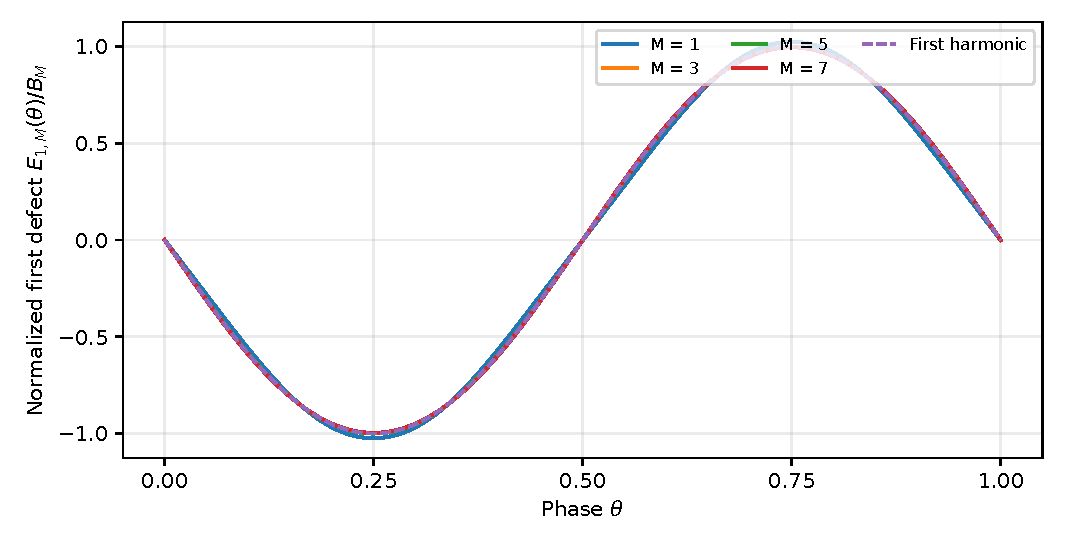
\includegraphics[width=0.94\linewidth]{figures/normalized_defect.pdf}
\caption{Normalized first defects for four odd mesh parameters, compared
with the reference harmonic $-\sin(2\pi\theta)$. Theorem
\ref{thm:complete-phases}, not the plot, proves that there are no other
zeros. The displayed curves use truncated Fourier series.}
\label{fig:phase}
\end{figure}

There is an elementary analytic truncation estimate for the product.
If $J$ is large enough that $|\pi t|2^{-J}\le1$, then all factors in the
tail starting at $J$ are positive and
\begin{equation}\label{eq:product-tail}
 0\le1-\prod_{j=J}^{\infty}\sinc(\pi t/2^j)
 \le\sum_{j=J}^{\infty}\frac{\pi^2t^2}{6\,4^j}
 =\frac{2\pi^2t^2}{9}\,4^{-J}.
\end{equation}
Here $1-\prod(1-a_j)\le\sum a_j$ for $a_j\in[0,1]$ is applied to
$1-\sinc(\pi t/2^j)$. For the normalized first-defect series, truncation
after an odd index $K$ has absolute error at most
$\sum_{k>K,\,k\text{ odd}}k^{-(p+2)}$, and relative error with respect to
$|\tau_p(\theta)|$ at most
$\sum_{k>K,\,k\text{ odd}}k^{-(p+1)}$. An interval implementation could
combine these estimates with directed rounding. The supplied numerical
program does not claim to do that.

\section{Integration with the formal repository}
\label{sec:formal}

\subsection{Existing dependencies and new obligations}

The inspected source already contains the Fourier-defect identity,
valuation-based alias vanishing, and sufficient parity-phase theorems
\cite{repo-phase,repo-defect}. In particular, the names
\begin{quote}\small\ttfamily
summable\_fourier\_monomialRvachevSchwartz\par
\medskip
tsum\_shifted\_monomial\_sub\_integral\par
\medskip
tsum\_shifted\_monomial\_sub\_integral\_odd\par
\medskip
tsum\_shifted\_polynomial\_eq\_integral\_superconvergent
\end{quote}
identify relevant existing declarations. The last theorem is a
\emph{sufficiency} theorem; its name alone should not be read as an
if-and-only-if statement.

A formalization of the new necessity proof can be broken into three
small analytic layers. First prove the sine multiple inequality and the
two exact quarter/half-integer factor ratios. Next pass the finite-product
ratio bound to the infinite product. Finally combine the odd defect series
with the weighted tail estimate, using the rational bound
$\delta_p<1/2$ if a zeta-function evaluation would add unnecessary
infrastructure. This yields completeness before the sharper constant is
formalized.

The phase-filter classification requires a second development: Fourier
coefficients of finite signed or complex measures on the circle, their
behavior under translation, and Fourier uniqueness. The finite atomic
case can be developed first, with direct finite sums, and then extended
to arbitrary finite measures. The orbit-count and budget proofs are
finite group-action arguments after the analytic exactness criterion.

The finite recognition theorem has an especially concrete formal route:
represent the difference between a measure and its translate by a finite
support list, establish its support-size bound, and use an invertible
Vandermonde matrix on distinct unit-circle points. This must not use real
conjugacy for complex weights; the two frequency ranges in
\cref{thm:finite-recognition} are genuinely different proof interfaces.

\subsection{A proposed theorem boundary}

For integer $M>0$, a natural formal endpoint is the equivalence
\[
 \bigl(\forall P\in\Poly_{\nu_2(M)+1},\ Q_{M,\theta}(P)=I(P)\bigr)
 \quad\Longleftrightarrow\quad \theta\bmod1\in Z_{\nu_2(M)+1}.
\]
The existing predicate uses explicit real representatives such as $0$ and
$1/2$. A new iff theorem must either work on the circle or explicitly
reduce $\theta$ modulo one. Otherwise, an assertion phrased for arbitrary
real $\theta$ would incorrectly exclude, for example, the phase $1$.

For rational $M=a/b$, the second endpoint should expose the \emph{reduced}
denominator $b$, not an arbitrary representation of the rational number.
At each degree it should connect uniform exactness to a cyclic-invariance
predicate of order $b2^{\max(0,r-\nu_2(a))}$. The phase-count theorem
must count active atoms after coalescing, not the length of a possibly
redundant input list.

No new formal file or checked theorem is included in this delivery. The
Python checks are not Lean certificates, and reading existing declarations
is not the same as rebuilding and auditing their dependencies. The article's
proofs stand independently as conventional proofs; formalization is a
well-specified next step rather than a completed claim.

\section{Further research questions and proposed projects}
\label{sec:research}

\subsection{Fixed-phase maximality beyond the first extra degree}

\textbf{Question 1.} For every integer $M>0$ and every
$\theta_0\in Z_p$, $p=\nu_2(M)+1$, is
$E_{p+1,M}(\theta_0)\ne0$? An affirmative answer would show that the
selected phases gain exactly one degree, not merely classify the phases
that gain at least one. The exact examples in \cref{tab:exact} support
this question but do not settle it. At the next degree, even aliases with
valuation one also enter, and derivatives of the nonvanishing product
tail occur at the odd aliases. The single first-harmonic estimate does
not directly resolve the resulting competition.

\subsection{Sharp domination constants and absolute conditioning}

\textbf{Question 2.} Determine the best universal constant in the
relative estimate \eqref{eq:relative-main}, or the sharp value of
\[
 \sup_{\substack{a,k\ge1\text{ odd}\\k\ge3}}
 k^2\frac{|H(ak/2)|}{|H(a/2)|}.
\]
The proof gives an upper bound of one for the latter, but the finite
experiment reaches only about $0.751$. Can long binary patterns in $a$
approach one, or is there a strict uniform improvement?

\textbf{Question 3.} Find effective upper and lower bounds on
$A_M=2p!|H(a/2)|/(2\pi M)^p$ in terms of the binary structure of $a$.
The current theorem gives mesh-independent \emph{relative} phase
conditioning. An absolute error tolerance requires control of $A_M$,
which can be very small. A useful result would separate the influence of
large $p$ from the small-divisor-like effects of the half-integer product.

\subsection{Stability of approximate Fourier invariance}

\textbf{Question 4.} Fix a support bound and a minimum separation between
active phases. If the moments in \cref{thm:finite-recognition} are only
approximately zero, how close must the filter be to a union of equal-weight
cyclic orbits? The Vandermonde proof suggests bounds involving the inverse
Vandermonde norm. A meaningful theorem should state the topology, weight
bounds, and separation assumptions explicitly: small finitely many
moments alone do not imply small total-variation distance to an invariant
measure.

\textbf{Question 5.} At meshes close to a rational $a/b$, quantify the
loss of uniform exactness for the optimal rational filter. The exact
rational/irrational dichotomy is discontinuous as a classification, while
finite-degree numerical errors vary continuously with the mesh. A
perturbation theorem could reconcile these two facts and give tolerances
for implementation.

\subsection{Other kernels, dimensions, and cost models}

\textbf{Question 6.} Which other compactly supported infinite-convolution
kernels admit a uniform first-coefficient ratio bound strong enough to
classify every first-superconvergent phase? For base-$q$ products, the
nonzero-frequency support may split into several residue classes rather
than just the odd integers. The zero multiplicities alone classify
uniform filters, but do not by themselves classify special-phase zeros.

\textbf{Question 7.} For a product of Rvachev kernels in several variables,
classify finite phase measures exact on total-degree polynomial spaces.
A non-product filter may exploit aliases killed by a zero in \emph{one}
coordinate. Thus the one-dimensional invariance theorem does not simply
imply that every optimal multidimensional filter is a product grid.
The correct obstruction is a multivariate set of derivative indices and
alias frequencies.

\textbf{Question 8.} How much can be saved when exactness is required at
one fixed phase instead of every translating phase? The exponential
phase-cost law proved here is tied to translation-uniformity. Allowing
phase-dependent weights or independent node positions changes the problem
and may permit substantially smaller formulas. A useful comparison would
retain a clearly specified lattice-mixture constraint while dropping only
the uniform-translation quantifier.

\subsection{Approximation theory and formal completion}

\textbf{Question 9.} Develop Peano-kernel or remainder estimates for
nonpolynomial smooth integrands at the classified phases. The leading
polynomial defect vanishes there, but an approximation theorem must also
control higher derivatives and the dependence of the weights on the
mesh. A sign-definite remainder formula would be particularly useful for
certified numerical integration.

\textbf{Question 10.} Complete a Lean formalization of the necessity
statement, then the atomic filter classification, then the general
measure version. The first target is comparatively focused: it can reuse
the existing odd-alias series and needs the relative product bound plus
an elementary convergent-series majorant. Formalizing the sharp zeta
constant can be separated from formalizing the qualitative result.

\section{Conclusion}

The missing phase-completeness statement has a quantitative answer: the
first defect cannot acquire additional zeros because its remaining odd
harmonics are uniformly dominated \emph{relative to} its first harmonic.
The resulting theorem holds for every integer mesh parameter, including
arbitrarily large odd parts.

At the level of translation-uniform phase mixtures, the answer is more
rigid. The reduced rational denominator and the dyadic valuation of the
numerator determine an exact cyclic symmetry group; that group determines
all admissible filters and their sharp finite cost. Irrational meshes
admit no finite filter even for uniform constant exactness. Minimum-size
and budget-optimal filters are necessarily ordinary uniform lattice
refinements, despite allowing signed or complex weights.

These results close a specifically documented repository gap and establish
a broader classification around it. Fixed-phase maximality at the next
degree, optimal constants, and multidimensional designs remain distinct,
precisely formulated problems.

\appendix
\section{A reusable first-harmonic zero-rigidity lemma}
\label{app:abstract}

The core argument does not intrinsically depend on the Rvachev function.
The following formulation isolates the transferable analytic mechanism.

\begin{proposition}[Odd-harmonic zero rigidity]\label[proposition]{prop:abstract}
Let $\varepsilon$ be either $0$ or $\pi/2$, let $a_1\in\R\setminus\{0\}$,
and let $(a_k)_{k\ge3,\,k\text{ odd}}$ be real coefficients such that
\[
 \eta=\frac1{|a_1|}\sum_{\substack{k\ge3\\k\text{ odd}}}k|a_k|<1.
\]
Then
\[
 f(x)=\sum_{\substack{k\ge1\\k\text{ odd}}}a_k\cos(kx+\varepsilon)
\]
has precisely the zeros of $\cos(x+\varepsilon)$, all simple, and
\[
 \left|\frac{f(x)}{a_1}-\cos(x+\varepsilon)\right|
 \le\eta|\cos(x+\varepsilon)|.
\]
At those zeros, $|a_1|(1-\eta)\le |f'(x)|\le|a_1|(1+\eta)$.
\end{proposition}
\begin{proof}
The weighted summability assumption gives uniform convergence of the
series and its first derivative. For odd $k$,
$|\cos(kx+\varepsilon)|\le k|\cos(x+\varepsilon)|$ by
\cref{lem:sine}. Summing the tail gives the displayed relative bound.
Since $\eta<1$, the sign and zero conclusions follow. At a reference
zero, the first derivative of the first term has absolute value $|a_1|$,
while the derivative tail has absolute value at most $\eta|a_1|$.
\end{proof}

For Rvachev quadrature, the coefficients normalized by their first term
satisfy $|a_k/a_1|\le k^{-(p+2)}$, making $\eta\le\delta_p$.
The factor $k$ in the weighted tail is not cosmetic. An unweighted small
tail controls the defect away from a reference zero, but need not prevent
additional zeros arbitrarily close to it.

\section{Reproducibility and the deliverable boundary}
\label{app:reproduce}

The archive contains this source, the compiled article, the figure assets,
the independent checking program, a saved JSON result, and build
instructions. From the archive root, run
\begin{quote}\ttfamily
python reproducibility/verify.py --plot
\end{quote}
to regenerate the diagnostic output and figure. The program requires
Python with \code{mpmath}; plotting additionally requires \code{numpy}
and \code{matplotlib}. The exact arithmetic uses only the standard
\code{fractions}, \code{math}, and \code{functools} modules.

Compile the article with
\begin{quote}\ttfamily
pdflatex -interaction=nonstopmode -halt-on-error article.tex\par
pdflatex -interaction=nonstopmode -halt-on-error article.tex\par
pdflatex -interaction=nonstopmode -halt-on-error article.tex
\end{quote}
The figure PDF is already included, so recompiling the article does not
require rerunning the numerical program. No external bibliography processor
is needed, and no font files are distributed.

The supplied exact checks validate finite identities and sample values.
The supplied numerical checks validate neither an infinite product nor an
infinite family of phases by themselves. The full statements are justified
by the analytic proofs in the main text. No changes were made to the
remote repository.

\begin{thebibliography}{9}
\raggedright
\bibitem{arias1982}
J. Arias de Reyna,
\emph{An infinitely differentiable function with compact support:
Definition and properties}, English translation (2017) of
\emph{Definici\'on y estudio de una funci\'on indefinidamente diferenciable
de soporte compacto}, Rev. Real Acad. Ciencias Madrid \textbf{76}
(1982), 21--38.
\url{https://arxiv.org/abs/1702.05442}.

\bibitem{arias2017}
J. Arias de Reyna,
\emph{Arithmetic of the Fabius function}, arXiv:1702.06487, version 3
(2017).
\url{https://arxiv.org/abs/1702.06487}.

\bibitem{zakharov2013}
V. G. Zakharov,
\emph{Polynomial spaces reproduced by elliptic scaling functions},
arXiv:1310.8425 (2013).
\url{https://arxiv.org/abs/1310.8425}.

\bibitem{repo-phase}
V. Reshetnikov and contributors,
\emph{ProveIt: RvachevSuperconvergentSynthesis.lean},
\path{Analysis/FabiusFunction/Lean/FabiusFunction/},
commit \texttt{de4ac5ab1438bcbeed58481c4449b593074a1a1f}.
\href{https://github.com/VladimirReshetnikov/ProveIt/blob/de4ac5ab1438bcbeed58481c4449b593074a1a1f/Analysis/FabiusFunction/Lean/FabiusFunction/RvachevSuperconvergentSynthesis.lean}{Pinned source file on GitHub}.
The introductory documentation states sufficient selected phases and
explicitly leaves their completeness unasserted.

\bibitem{repo-defect}
V. Reshetnikov and contributors,
\emph{ProveIt: CombDefectSeries.lean},
\path{Analysis/FabiusFunction/Lean/FabiusFunction/},
commit \texttt{de4ac5ab1438bcbeed58481c4449b593074a1a1f}.
\href{https://github.com/VladimirReshetnikov/ProveIt/blob/de4ac5ab1438bcbeed58481c4449b593074a1a1f/Analysis/FabiusFunction/Lean/FabiusFunction/CombDefectSeries.lean}{Pinned source file on GitHub}.
The source gives absolutely convergent defect series and odd-frequency
support at the first threshold.
\end{thebibliography}
\end{document}
